% =========================================================================
% SciPost LaTeX template
% Version 1e (2017-10-31)
% =========================================================================
%\documentclass[submission, Proceedings]{SciPost}

%-------------------------------------------------
% CERN-LHC-CMS specific styles
%-------------------------------------------------
\newcommand{\Pmu}{\ensuremath{{\PGm}}\xspace}
\newcommand{\pzvar}{\ensuremath{p_\text{Z}(\Pepm, \PGmmp, j)}\xspace}
\newcommand{\invmassvar}{\ensuremath{m(\Pepm, \PGmmp,j)}\xspace}
\newcommand{\transmassvar}{\ensuremath{m_{\text{T}}(\Pepm, \PGmmp,j,\ptmiss)}\xspace}
\newcommand{\deltaPhiVar}{\ensuremath{\Delta\varphi(\Pepm, \PGmmp)}\xspace}
\newcommand{\ljets}{\ensuremath{\ell + \text{jets}}\xspace}
\newcommand{\dilep}{\ensuremath{2\ell + \text{jets}}\xspace}
\newcommand{\ttjets}{\ensuremath{\ttbar + \text{jets}}\xspace}
\newcommand{\ttgamma}{\ensuremath{\ttbar\gamma}\xspace}
\newcommand{\cc}{\ensuremath{\PQc\PAQc}\xspace}
\newcommand{\bb}{\ensuremath{\PQb\PAQb}\xspace}
\newcommand{\ttcc}{\ensuremath{\ttbar\PQc\PAQc}\xspace}
\newcommand{\ttcL}{\ensuremath{\ttbar\PQc\text{L}}\xspace}
\newcommand{\ttbb}{\ensuremath{\ttbar\PQb\PAQb}\xspace}
\newcommand{\ttbL}{\ensuremath{\ttbar\PQb\text{L}}\xspace}
\newcommand{\ttLF}{\ensuremath{\ttbar\text{LL}}\xspace}
\newcommand{\ttjj}{\ensuremath{\ttbar\text{jj}}\xspace}
\newcommand{\mujets}{\ensuremath{\PGm + \text{jets}}\xspace}
\newcommand{\ejets}{\ensuremath{\Pe + \text{jets}}\xspace}
\newcommand{\tW}{\ensuremath{\PQt\PW}\xspace}

\binoppenalty=10000
\relpenalty=10000

\hypersetup{
    colorlinks,
    linkcolor={red!50!black},
    citecolor={blue!50!black},
    urlcolor={blue!80!black}
}

%%\usepackage[bitstream-charter]{mathdesign}
\urlstyle{sf}

% Fix \cal and \mathcal characters look (so it's not the same as \mathscr)
%%\DeclareSymbolFont{usualmathcal}{OMS}{cmsy}{m}{n}
%%\DeclareSymbolFontAlphabet{\mathcal}{usualmathcal}

%%\begin{document}

%\linenumbers
\begin{center}{\Large \textbf{
            Top quark pair and single top cross sections and ttX (CMS)\\
}}\end{center}
\begin{center}
Ravindra K Verma on behalf of the CMS Collaboration\textsuperscript{$\star$} 
\end{center}
\begin{center}
Florida Institute of Technology, USA 
\\
*rverma@cern.ch 
\end{center}
\begin{center}
\today
\end{center}

\definecolor{palegray}{gray}{0.95}
\begin{center}
\colorbox{palegray}{
  \begin{tabular}{rr}
  \begin{minipage}{0.1\textwidth}
    
\includegraphics[width=22mm]{Logo-DIS2021.png}
  \end{minipage}
  &
  \begin{minipage}{0.75\textwidth}
    \begin{center}
    {\it Proceedings for the XXVIII International Workshop\\ on Deep-Inelastic Scattering and
Related Subjects,}\\
    {\it Stony Brook University, New York, USA, 12-16 April 2021} \\
    \doi{10.21468/SciPostPhysProc.?}\\
    \end{center}
  \end{minipage}
\end{tabular}
}
\end{center}


\section*{Abstract}
{\bf
Latest results on inclusive and differential \PQt quark pairs, single \PQt, and {\ttbar}X 
production cross sections are presented using proton-proton collision data collected by the CMS 
experiment. The differential cross sections are measured as a function of various kinematic 
observables of the \PQt quarks, jets, and leptons of the event final state. The results are 
confronted with precise theory calculations and used to constrain Standard Model parameters. 
Measurements are also performed with high transverse momentum of the \PQt quarks, i.e., in the 
boosted regimes.
%Measurements of the cross section for the production of the single top with a \PW boson, top quark 
%pairs with and without additional quarks are presented at the different center of mass energies 
%with different integrated luminosity recorded by the CMS experiment during the years 2016-18 of 
%data-taking. The 
%measurement is performed in semi and dileptonic decay modes of the top quark. A few of them 
%are performed for the first time. The measured and the predicted value of the inclusive cross 
%section are in agreement within the uncertainties. The differential and double differential
%measurement has slight over-prediction in a certain kinematic region due to the mismodeling of 
%the event generator.
}


\section{Introduction}
\label{sec:intro}
The top quark is one of the most interesting particles present in the Standard Model (SM) of
particle physics as it is postulated to interact with unknown particles from theories beyond the 
SM because of its high mass. Precise measurement of the properties of the top quark helps in the 
improvement of search sensitivity and test of perturbative Quantum Chromodynamics. Differential 
cross section measurements are used to test fixed-order predictions and extract QCD parameters. 
The \ttbar production is dominant at LHC and serves as the background for many new physics searches.

There have been many earlier measurements at 7, 8, and 13 \TeV center-of-mass energy 
as shown in Figure~\ref{fig:xss}. 
In this proceeding, we summarise the recent cross section measurements by the CMS experiment at the
LHC. For a more detailed description of each of the measurements, the reader is encouraged to look
at the corresponding paper. Here we summarise the \ttbar measurements in Section~\ref{sec:tt},
\tW in Section~\ref{sec:tW}, and $\ttbar$X in Section~\ref{sec:ttX} where X stands for 
\text{$\gamma$}, \cc, and \bb.

\begin{figure}[htb!]
\centering
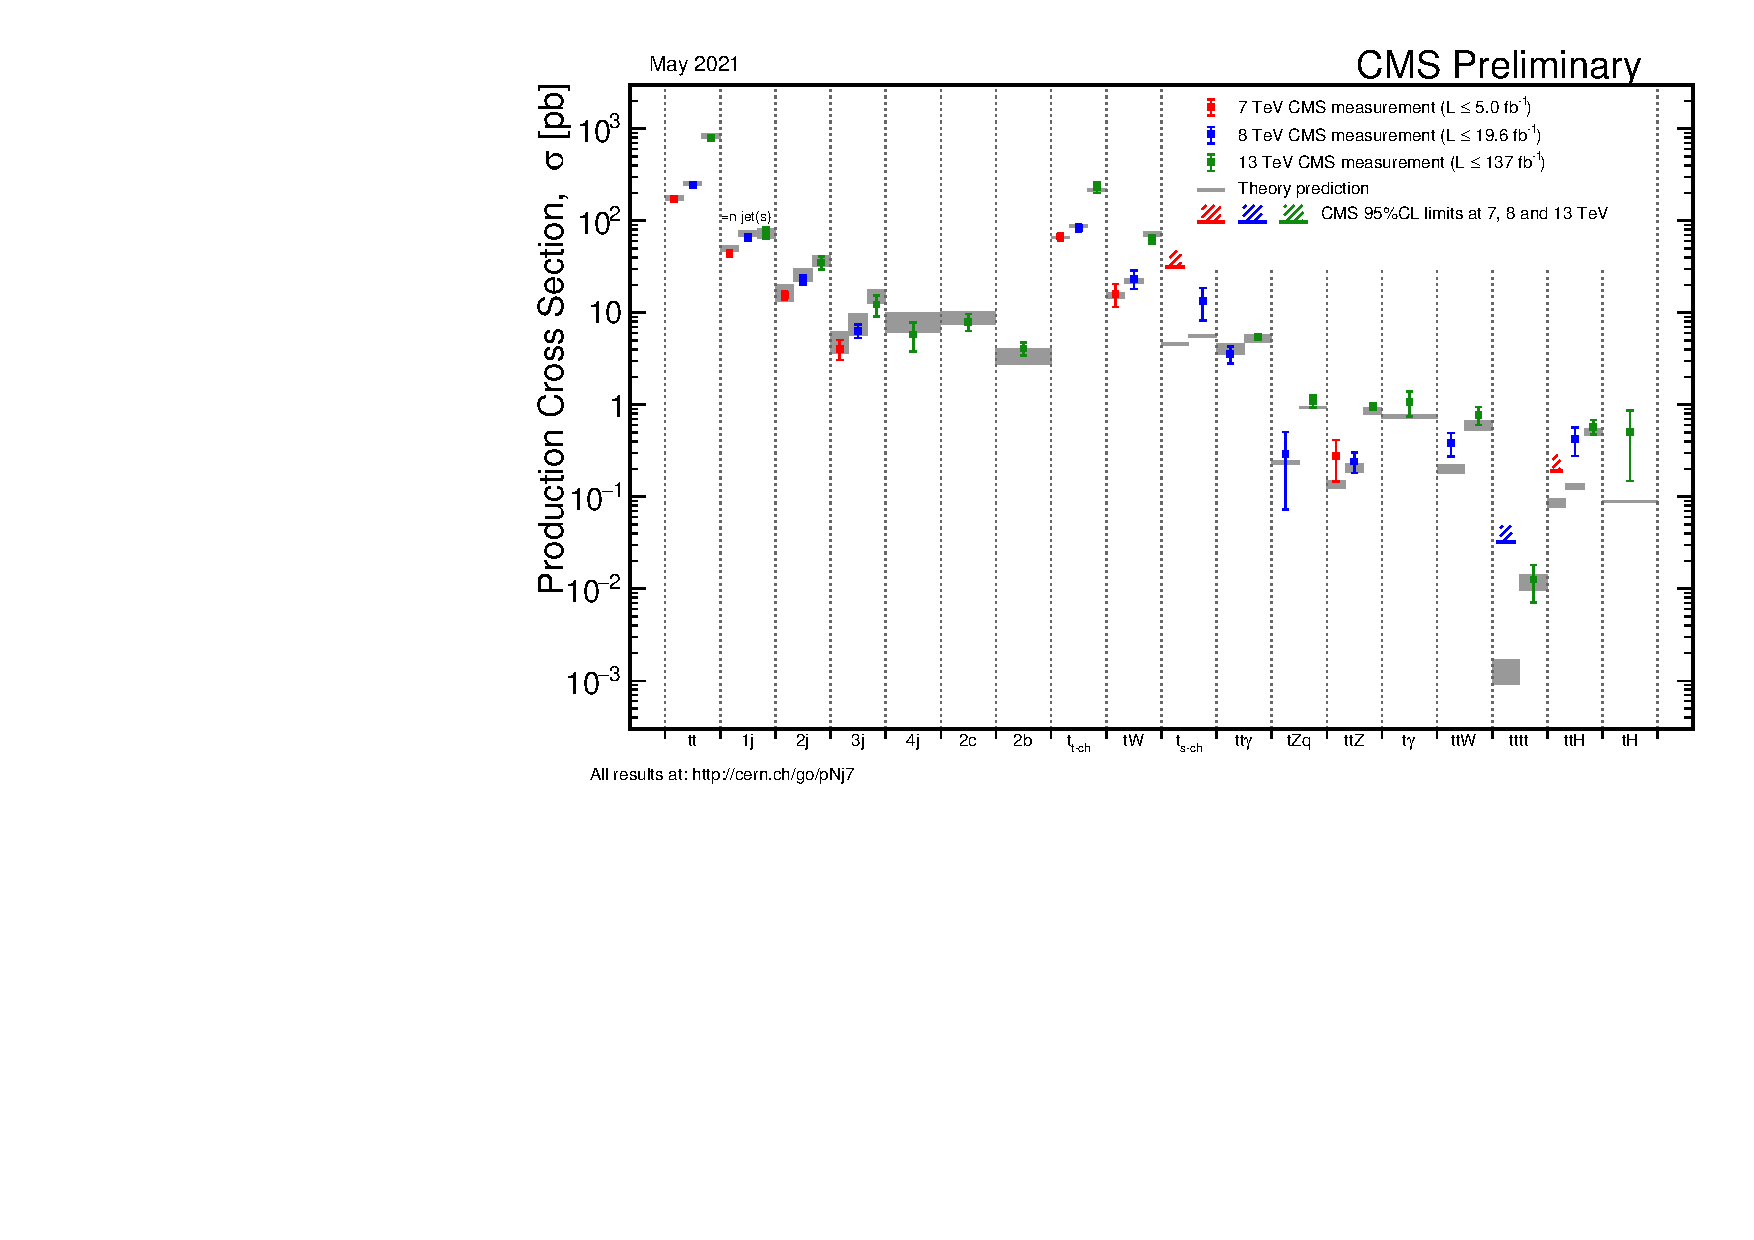
\includegraphics[width=1.0\linewidth]{SigmaNew_v8.pdf}
\caption{Top quark production cross section at various center-of-mass energies measured by the
	CMS experiment. The measurements are performed for the production of single \PQt, \ttbar, \ttbar + jets, \PQt + X, \ttbar+ X, \ttbar\ttbar, etc. Among these, a few of them are new at 13 \TeV whereas a
	few of them are still being studied. There is a good agreement between the predicted and
	measured values within the uncertainties.}
\label{fig:xss}
\end{figure}



\section{\texorpdfstring{\ttbar}{ttbar} production}
%================
% tt
%================
Due to the higher cross section among all \PQt quark production processes, the \ttbar production process is extensively studied at the LHC.
Depending on the subsequent decays of the two \PQt quarks, the final states consist of either all
jets, \ljets, or \dilep. All-jet final states have larger size of the selected data set but more 
multijet background whereas the \dilep final states have fewer events but small background. The \ljets 
final states fall in between the two. However, the measurement of cross sections from all these 
final states is needed in order to study various physics beyond the SM. In these proceedings, we 
present the measurement from the \ljets and \dilep final states for \ttbar production.


\subsection{Inclusive and differential cross section measurements in the \texorpdfstring{\ljets}{ljets} final states}
The measurement of the \ttbar cross section is performed using 137 \fbinv integrated luminosity in 
the \ejets and \mujets final states~\cite{CMS-PAS-TOP-20-001}. In order to increase the 
sensitivity, the events are further divided into boosted and resolved categories based on the 
kinematics of the decay products of the \ttbar pair. The final cross section is extracted by a 
simultaneous fit combining events from both final states and all categories. Various distributions 
such as the transverse momentum of the \PQt quark, invariant mass of \ttbar, etc are used to 
measure the differential and double differential cross-sections at parton and particle levels. A 
neural network is exploited in the reconstruction of variables from boosted \PQt quarks. 
A $\chi^2$ test is performed to compare the measurements with several predictions. The dominant 
source of systematic uncertainty comes from jet energy correction.

The measured value of the inclusive cross section, $791\pm 25$ pb, is in agreement with the corresponding 
predicted value of $832\pm 46$ pb. One of the most 
striking features of this measurement is that the measured cross section is more precise 
(3.2\% uncertainty) as compared to the predicted value (5.5\% uncertainty). The measured and 
predicted differential and double differential cross sections as functions of various variables are 
in agreement within the uncertainties for most of the variables. However, there is a slight 
discrepancy in the double differential measurement for higher \pt of the hadronically decaying \PQt
quark in the range $ 0 < \pt (\ttbar) < 120 \GeV$. A similar over-prediction is 
also observed from the ATLAS experiment~\cite{ATLAS:2020ccu} and signals a possible mismodeling 
of the Monte Carlo event generator used for the simulation of predicted events. 

\subsection{Inclusive cross section measurement in the \texorpdfstring{\dilep}{dilep} final states at 5.02 \texorpdfstring{\TeV}{TeV} center-of-mass energy}
As shown in Figure~\ref{fig:xss}, all measurements are performed at 7, 8, and 13 \TeV center-of-mass 
energies. This is the first measurement at 5.02 \TeV, which provides another test for the 
SM at lower energy~\cite{CMS-PAS-TOP-20-004}. The measurement is performed using 0.304\fbinv 
integrated luminosity in the \ejets and \mujets final states. The cross section is extracted 
by performing the fit on the total number of events after applying all selections. The dominant source 
of systematic uncertainty comes from the jet energy correction. The predicted cross section at the
next-to-leading order (NLO) in QCD and observed value are 
$66.8^{+1.9}_{-2.3}\text{(scale)}\pm 1.7\text{(PDF)}^{+1.4}_{-1.3}(\alpha_S)$ pb and 
$60.3 \pm 5.0 \text{(stat)} \pm 2.8 \text{(syst)} \pm 0.9 \text{(lumi)}$ pb, respectively. They
agree within the uncertainties. 

\subsection{Inclusive cross section measurement in the \texorpdfstring{\dilep}{dilep} final states including \texorpdfstring{\PGt}{tau} lepton}
This is the first measurement involving tau leptons~\cite{CMS:2019snc} and provides another 
way of checking lepton flavor universality. With the third generation of lepton and quarks,
it is sensitive to beyond SM contributions such as the production of charged Higgs boson. In 
this analysis, one of the leptons from \dilep final states is required to be a hadronically 
decaying \PGt and the other one is either an electron or muon. The measurement is performed at 
13 \TeV using 35.9\fbinv integrated luminosity. The cross section is extracted using the profile 
likelihood method based on the transverse mass of the lepton and missing transverse energy. The  
QCD multijet background is estimated from data. The main sources of systematic uncertainty are 
from $\tau_h$ identification and misidentification. The measured cross section combining both 
channels is  
$\sigma_\ttbar(\ell\tau_h) = 781 \pm 7 \text{(stat)} \pm 62 \text{(syst)} \pm 20 \text{(lumi)}$ pb, 
which is in agreement with the corresponding predicted value. The ratio of this with the same 
flavor cross section 
$R_{\ell\tau_h/\ell\ell} = 0.973 \pm 0.009 \text{(stat)} \pm 0.066 \text{(syst)}$ is close to 1 
within the uncertainties. Hence the lepton flavor universality violation is not observed.


\label{sec:tt}

\section{\texorpdfstring{\tW}{tW} production} 
 %================
 % tW
 %================
 The \tW production process is one of the sub-dominants in terms of the total cross section as 
 shown in Figure~\ref{fig:xss}. It is also sensitive to the relevant CKM matrix element. 
 Any deviation from the predicted value may be indicative of physics beyond the SM. Similar to the 
 \ttbar measurement, we present the recent studies from the \ljets and \dilep final states.

 \subsection{Inclusive cross section measurement in the \texorpdfstring{\ljets}{ljets} final states}
 The measurement is performed in the \ejets and \mujets final states with 35.9\fbinv integrated
 luminosity~\cite{CMS-PAS-TOP-20-002}. An event-level discriminant based on Boosted Decision Tree 
 is used to extract the cross section. The events are divided into different signal and control 
 regions based on the number of jets and b-tagged jets. A simultaneous fit is performed on the
 discriminant combining 3 categories and 2 final states. The dominant source of systematic 
 uncertainty comes from the jet energy correction. The predicted (at NLO) and 
 measured cross sections are $79.5^{+1.9+2.0}_{-1.8-1.4}$ pb and 
 $89 \pm 4 (\text{stat}) \pm 12 (\text{syst})$ pb, respectively. They are in agreement within the
 uncertainties.

 \subsection{Differential cross section measurement in the \texorpdfstring{\dilep}{dilep} final states}
 The differential cross section is measured with 35.9\fbinv integrated luminosity in the \dilep final
 states with different lepton flavors (electron or muon) as a function of the six 
 variables~\cite{CMS-PAS-TOP-19-003}: \pt of the leading lepton, \pt of the jet, angular difference
 \deltaPhiVar, longitudinal momentum \pzvar, invariant mass \invmassvar, and transverse mass 
 \transmassvar. Signal extraction is performed by subtracting backgrounds from data. The jet energy 
 correction uncertainties are the dominant ones. Predicted and measured cross sections are in 
 agreement within the uncertainties across different bins of all variables.

\label{sec:tW}

\section{\texorpdfstring{\ttgamma, \ttcc, \ttbb}{ttXX} productions}
 %================
 % ttX
 %================
 Although the cross sections of these processes are smaller as shown in Figure~\ref{fig:xss},
 they are useful in studying rare phenomena within the SM and new physics beyond it, for example, 
 the \ttgamma measurement allows in constraining the $\PQt\gamma$ electroweak coupling and $\ttcc$ or
 \ttbb provide a useful test of NLO QCD calculations. 

 \subsection{Inclusive and differential \texorpdfstring{\ttgamma}{ttgamma} cross section measurements in \texorpdfstring{\ljets}{ljets} final states}
 This is the first \ttgamma cross section measurement at 13 \TeV by the CMS experiment using 137\fbinv
 integrated luminosity~\cite{CMS-PAS-TOP-18-010}. The measurement is performed in the \ejets and 
 \mujets final states with one photon. Photons are classified based on matched generator parton in 
 the genuine, nonprompt, misidentified, and multijet photon categories. Different phase spaces based 
 on object selections and kinematic cuts are exploited to improve the precision. QCD multijet and 
 electroweak backgrounds are measured from data. A simultaneous fit combining all event categories is 
 performed to extract the cross section. The dominant uncertainties in the cross section comes from 
 $\PW\gamma$ normalization and misidentified $\gamma$ estimation. The measured value of the inclusive
 cross section in  the fiducial phase space is $800 \pm 46 (\text{syst}) \pm 7 (\text{stat})$ fb.
 The ratio of the measured and predicted (at NLO) cross section is $1.034^{+0.060}_{-0.058}$,
 that is, they agree within the uncertainties. There is also good agreement for the differential 
 cross section in most bins of \pt and $\eta$ of the photon. Though there is a slight over-prediction
 in the bins where statistical precision is low. 

 \subsection{Inclusive \texorpdfstring{\ttcc}{ttcc} cross section measurement in \texorpdfstring{\dilep}{dilep} final states}
 Due to the availability of \PQc-jet taggers at 13 \TeV, there has been an improvement in the 
 sensitivity in the measurement involving \PQc jet in the final state. For the first time, a \ttcc 
 cross section measurement is performed  by the CMS Collaboration~\cite{CMS-PAS-TOP-20-003}. The 
 analysis is performed in the \dilep final states with the same flavor lepton (\Pe, \Pmu, or \PGt) 
 with 41.5\fbinv integrated luminosity at the center-of-mass energy of 13 \TeV. A neural network is 
 trained to distinguish between top quark pair events with additional jets. Event level neural 
 network predicts output probabilities for five output classes $P$($\ttcc$), $P$($\ttcL$), $P$($\ttbb$), $P$($\ttbL$), and $P$($\ttLF$). Two variables are derived based on these
 \begin{linenomath}
 \begin{equation}
   \begin{aligned}
 \Delta_{\PQb}^{\PQc} &= \frac{P(\ttcc) }{P(\ttcc) + P(\ttbb)},\\
 \Delta_{\text{L}}^{\PQc} &=  \frac{P(\ttcc)}{P(\ttcc) + P(\ttLF)}.
 \label{eq:Dbcdiscriminator}
   \end{aligned}
 \end{equation}
 \end{linenomath}
 A 1-d histogram is constructed from the 16 bins of the 2-d plane of these two variables
 \begin{equation}
 \Delta_{\text{L}}^{\PQc} \otimes \Delta_{\PQb}^{\PQc} :  [0,0.55,0.65,0.85,1.0] \otimes [0,0.35,0.5,0.6,1.0].
 \end{equation}
 The \ttcc, \ttbb, \ttLF cross sections are simultaneously extracted by fitting the neural network
 outputs from simulation and observation. The dominant source of systematic uncertainty comes 
 from the jet energy correction and c-tagging calibration. The $\ttcc$ cross section in the
 full phase space is measured to be $7.43\pm 1.07(\text{stat})\pm 0.95(\text{syst})$ pb. 
 An overall agreement is observed between the measured and predicted value at the level of 
 one to two standard deviations for the \ttcc, \ttbb, and \ttLF processes. 

 \subsection{Inclusive \texorpdfstring{\ttbb}{ttbb} cross section measurements in \texorpdfstring{\ljets}{ljets} and \texorpdfstring{\dilep}{dilep} final states}
 The measurement is performed at 13 \TeV with 35.6\fbinv integrated luminosity~\cite{CMS:2020grm}. 
 The cross section is separately extracted for both final states for \ttbar and \ttjj and their ratio
 in the visible and full phase space. The fit is performed on the b-tagging discriminant value of 
 the two jets. A 1-d histogram is constructed from the 10x10(20x20) bins of the 2-d plane of these 
 two variables for \ljets (\dilep) final states. Theoretical uncertainties from the final state
 radiation and madevent parton-shower matching are dominant. The corresponding measured cross
 section for \ttbb in the full phase space is $4.7 \pm 0.2 (\text{stat}) \pm 0.6 (\text{syst})$ pb 
 and $2.9 \pm 0.1 (\text{stat}) \pm 0.5 (\text{syst})$ pb for \ljets and \dilep final states, 
 respectively. These are consistent within the uncertainties, with the SM prediction obtained using 
 a matrix element calculation at NLO order in QCD matched to a parton shower.

 \section{Conclusion}
 In this proceedings, a summary of the inclusive, differential, and double differential cross section
 measured by the CMS experiment is presented for different final states. The measured value of 
 \ttbar cross section is more precise as compared to the predicted one. A slight over-prediction
 is seen in the differential \ttgamma due to low statistics and double differential \ttbar cross 
 section due to mismodeling of the \pt spectrum of the \ttbar system. The \ttbar measurement at
 5.02 \TeV provides another way of testing the consistency of SM prediction with the observation
 at lower energy. For the first time, the final states involving \PGt lepton are analyzed for the
 \ttbar process. Other measured cross sections for the \PQt\PW, \ttgamma, \ttcc and \ttbb 
 production processes are in agreement with SM prediction within the systematic and statistical 
 uncertainties.


\label{sec:ttX}

%\begin{verbatim}
%\bibliographystyle{SciPost_bibstyle}
\bibliography{auto_generated}
%\end{verbatim}
